\chapter{Dữ liệu về điện tim}
\newpage

\section{Physionet}
\subsection{Thông tin về dataset}
Là một trang web truy cập miễn phí các bộ dữ liệu lớn về tín hiệu sinh lý được ghi lại (PhysioBank) và những phần mềm mã nguồn mở liên quan (PhysioToolkit).
\begin{center}
    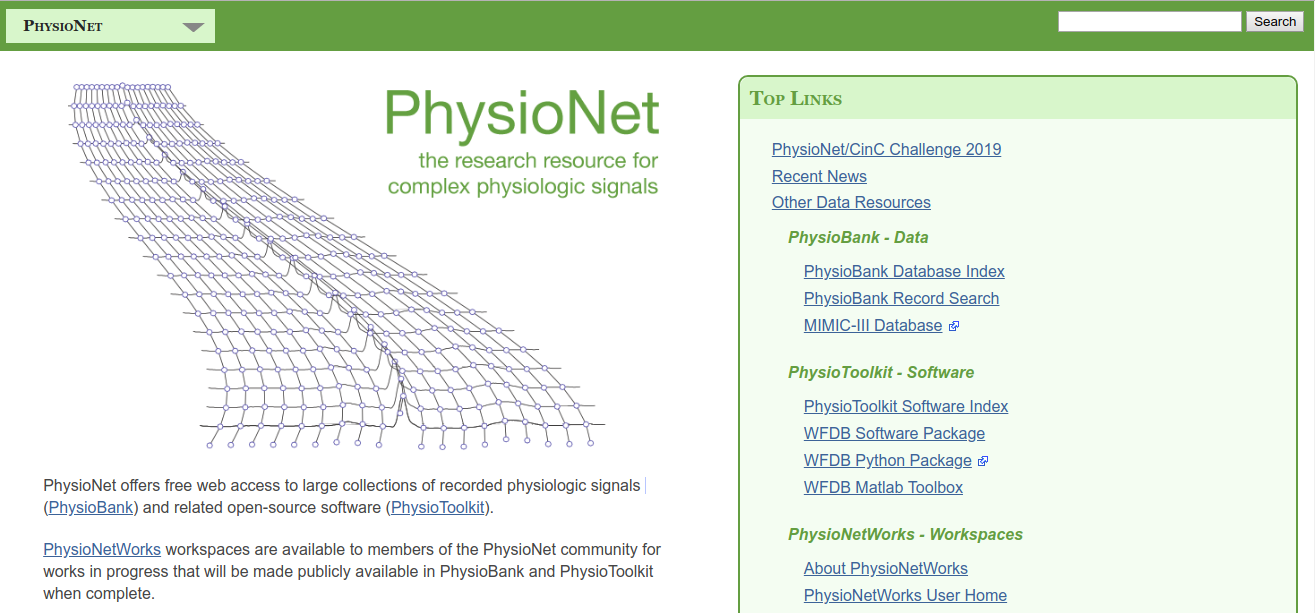
\includegraphics[scale=.3]{image/chapter3/Screenshot_from_2019-03-11_04-58-18.png}
    \begin{figure}[htp]
    \begin{center}
    \end{center}
    \caption{Trang Physionet}
    \end{figure}
\end{center}

\subsection{MIT-BIH Arrhythmia Database}
\textbf{Thông tin về database}
Đây là bộ dữ liệu nổi tiếng nhất, nhiều bài báo cũng như nghiên cứu dựa trên bộ dữ liệu này. Tập dữ liệu bao gồm 48 file. Mỗi file gồm: 1 file dat chứa dữ liệu, một file atr chứa chú thích, 1 file hea chứa header.
\begin{center}
    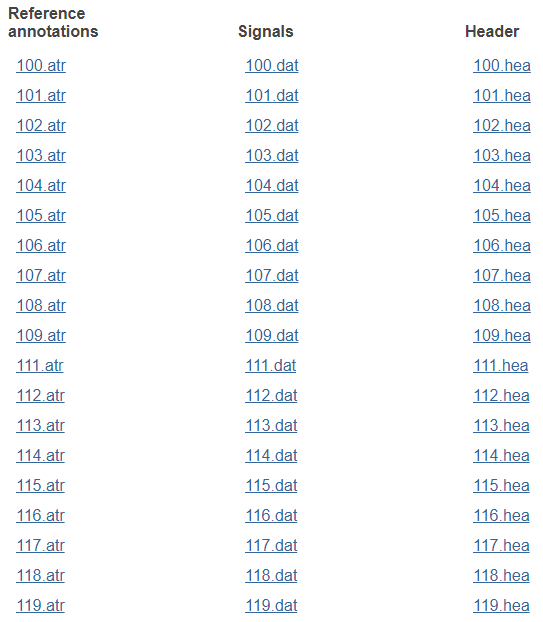
\includegraphics[scale=.4]{image/week3/mit.png}
    \begin{figure}[htp]
    \begin{center}
    \end{center}
    \caption{Dataset sample}
    \end{figure}
\end{center}
Phân tích và plot file 100.mat thành đồ thị.
\begin{center}
    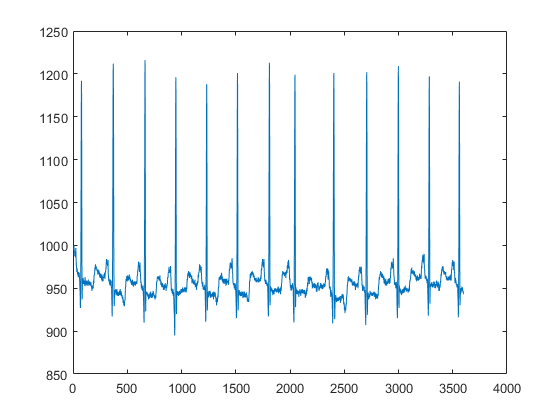
\includegraphics[scale=.8]{image/week4/100dat.png}
    \begin{figure}[htp]
    \begin{center}
    \end{center}
    \caption{100.mat sau khi plot thành đồ thị thể hiện hình dạng ECG}
    \end{figure}
\end{center}
